% Differential power processing (DPP) for photovoltaic string
% For more details refer to: https://doi.org/10.1109/TEC.2018.2876176  --> (Review of Differential Power Processing Converter Techniques for Photovoltaic Applications)
%Designed by: Amir Ostadrahimi
\documentclass[border=5pt,tikz]{standalone}
\usepackage[american,cuteinductors,smartlabels]{circuitikz}
\ctikzset{bipoles/thickness=1.2}
\ctikzset{bipoles/length=1cm}
\ctikzset{bipoles/diode/height=.25}
\ctikzset{bipoles/diode/width=.2}
\tikzstyle{every node}=[font=\small]
\tikzstyle{every path}=[line width=0.8pt,line cap=round,line join=round]

\begin{document}
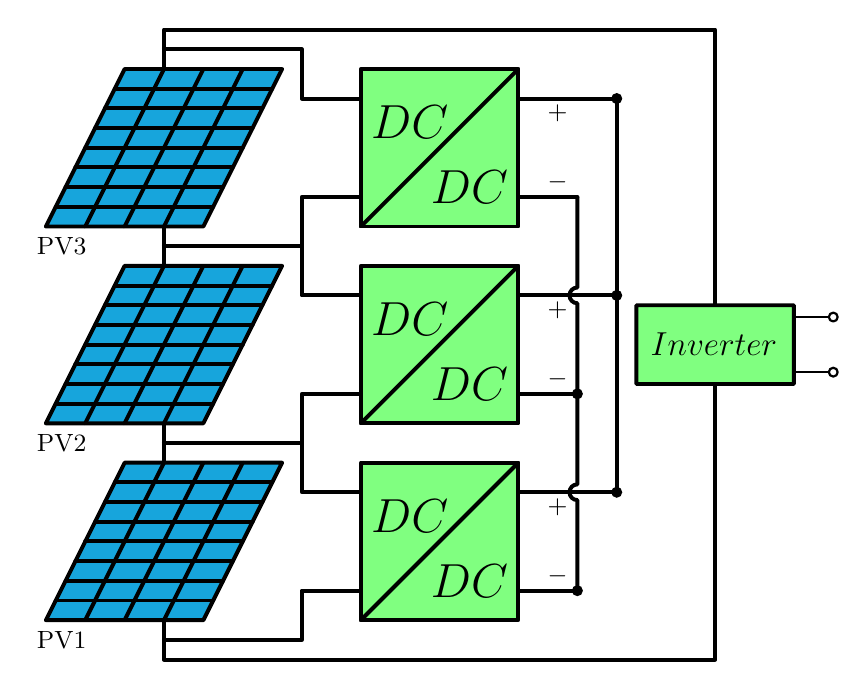
\begin{tikzpicture}

% Part 1; General topology
%Panel1
	%Frame
	\draw (0,0) coordinate (P1);
	\draw (P1)++(2,0) coordinate(P2);
	\draw (P1)++(-1,-2) coordinate (P3);
	\draw (P3)++(2,0) coordinate(P4);
	\draw [line width=.5mm, fill=cyan!90!black] (P1)--(P2)--(P4)--(P3)--cycle;
	%Horizontal Lines
	\draw [line width=.5mm] (P1)++ (-.125,-0.25)--(1.875,-.25) ;
	\draw [line width=.5mm] (P1)++ (-.25,-0.5)--(1.75,-.5)  ;
	\draw [line width=.5mm] (P1)++ (-.375,-0.75)--(1.625,-.75) ;
	\draw [line width=.5mm] (P1)++ (-.5,-1)--(1.5,-1) ;
	\draw [line width=.5mm] (P1)++  (-.625,-1.25)--(1.375,-1.25) ;
	\draw [line width=.5mm] (P1)++ (-.75,-1.5)--++(2,0)  ;
	\draw [line width=.5mm] (P1)++  (-.875,-1.75)--++(2,0) coordinate (P34) ;
	%Vertical Line
	\draw [line width=.5mm] (.5,0)--++(-1,-2);
	\draw [line width=.5mm] (1,0)--++(-1,-2);
	\draw [line width=.5mm] (1.5,0)--++(-1,-2);
	\draw (P3)++(0.2,-0.25) coordinate (Pname);
	\node (PVname) at (Pname) {PV1};
	%connections in the bottom and top of the panel
	\draw (P3)++(1.5,0) coordinate(PV1in);
	\draw (P1)++(0.5,0) coordinate(PV1out);
	%Converter
	\draw [line width=.5mm] (P2)++(1,0) coordinate(C1);
	\draw (C1)++(2,0) coordinate (C2);
	\draw (C1)++(0,-2) coordinate (C3);
	\draw (C3)++(2,0) coordinate (C4);
	\draw  [line width=.5mm, fill=green!50] (C1)-- (C3)--(C4)--(C2)--cycle;
	\draw [line width=.5mm] (C3)--(C2);
	%
	\draw (1.8125,-.375)  coordinate(conn1) ;
	\draw (P4)++(.125,.25)--++(.0625,.125) coordinate(conn2) ;
	\draw (conn1)++(.1,-.05) coordinate(VPV);
	%Connection of Panel and coverter
	\draw (conn1-|C1) coordinate(connC1);
	\draw (conn2-|C1) coordinate(connC2);
	%
	\draw (connC1)++(2,0) coordinate (connC3);
	\draw (connC2)++(2,0) coordinate (connC4);
	%
	\draw (C2)++(0,-1) coordinate (CM); %middle of converter at right side
	%parallell
	\draw [line width=.5mm] (connC3)--++(0.5,0) coordinate(OutUp1)--++(0.75,0) coordinate(OutParallel1u);
	\draw [line width=.5mm] (connC4)--++(0.5,0) coordinate(OutBt1)--++(0.25,0) coordinate (OutParallel1b);
	\fill (OutParallel1u) circle (2pt);
	\fill (OutParallel1b) circle (2pt);
	\draw  (OutUp1) to [open, v=$ $](OutBt1);
	\draw (connC1)++(0,-.3) coordinate (T1);
	\node [below, right](Text1) at (T1) {\LARGE $DC$}; 
	\draw (C4)++(0,0.5) coordinate (T2);
	\node [above, left](Text1) at (T2) {\LARGE$ DC$}; 
%Panel2
	%Frame
	\draw (0,2.5) coordinate (P1-2);
	\draw (P1-2)++(2,0) coordinate(P2-2);
	\draw (P1-2)++(-1,-2) coordinate (P3-2);
	\draw (P3-2)++(2,0) coordinate(P4-2);
	\draw [line width=.5mm, fill=cyan!90!black] (P1-2)--(P2-2)--(P4-2)--(P3-2)--cycle;
	%Horizontal Lines
	\draw [line width=.5mm] (P1-2)++ (-.125,-0.25)--++(2,0) ;
	\draw [line width=.5mm] (P1-2)++ (-.25,-0.5)--++(2,0)   ;
	\draw [line width=.5mm] (P1-2)++ (-.375,-0.75)--++(2,0)  ;
	\draw [line width=.5mm] (P1-2)++ (-.5,-1)--++(2,0)  ;
	\draw [line width=.5mm] (P1-2)++  (-.625,-1.25)--++(2,0)  ;
	\draw [line width=.5mm] (P1-2)++ (-.75,-1.5)--++(2,0)  ;
	\draw [line width=.5mm] (P1-2)++  (-.875,-1.75)--++(2,0) coordinate (P34-2) ;
	%Vertical Line
	\draw [line width=.5mm] (P1-2)++(.5,0)--++(-1,-2);
	\draw [line width=.5mm](P1-2)++ (1,0)--++(-1,-2);
	\draw [line width=.5mm] (P1-2)++(1.5,0)--++(-1,-2);
	\draw (P3-2)++(0.2,-0.25) coordinate (Pname-2);
	\node (PVname-2) at (Pname-2) {PV2};
	%connections in the bottom and top of the panel
	\draw (P3-2)++(1.5,0) coordinate(PV2in);
	\draw (P1-2)++(0.5,0) coordinate(PV2out);
	%Converter
	\draw [line width=.5mm] (P2-2)++(1,0) coordinate(C1-2);
	\draw (C1-2)++(2,0) coordinate (C2-2);
	\draw (C1-2)++(0,-2) coordinate (C3-2);
	\draw (C3-2)++(2,0) coordinate (C4-2);
	\draw  [line width=.5mm, fill=green!50] (C1-2)-- (C3-2)--(C4-2)--(C2-2)--cycle;
	\draw [line width=.5mm] (C3-2)--(C2-2);
	%
	\draw (P1-2)++ (1.8125,-.375)  coordinate(conn12) ;
	\draw (P4-2)++(.125,.25)--++(.0625,.125) coordinate(conn22) ;
	\draw (conn12)++(.1,-.05) coordinate(VPV-2);
	%Connection of Panel and coverter
	\draw (conn12-|C1-2) coordinate(connC1-2);
	\draw (conn22-|C1-2) coordinate(connC2-2);
	%
	\draw (connC1-2)++(2,0) coordinate (connC3-2);
	\draw (connC2-2)++(2,0) coordinate (connC4-2);
	%
	\draw (C2-2)++(0,-1) coordinate (CM2); %middle of converter at right side
	%parallell
	\draw [line width=.5mm] (connC3-2)--++(0.5,0) coordinate(OutUp2)--++(0.75,0)coordinate(OutParallel2u);
	\fill (OutParallel2u) circle (2pt);
	\draw [line width=.5mm] (connC4-2)--++(0.5,0) coordinate(OutBt2)--++(0.25,0) coordinate (OutParallel2b);
	\fill (OutParallel2b) circle (2pt);
	\draw  (OutUp2) to [open,v=$ $](OutBt2);
	\draw (connC1-2)++(0,-.3) coordinate (T1-2);
	\node [below, right](Text1-2) at (T1-2) {\LARGE $DC$}; 
	\draw (C4-2)++(0,0.5) coordinate (T2-2);
	\node [above, left](Text1-2) at (T2-2) {\LARGE$ DC$}; 
%Panel3
	%Frame
	\draw (0,5) coordinate (P1-3);
	\draw (P1-3)++(2,0) coordinate(P2-3);
	\draw (P1-3)++(-1,-2) coordinate (P3-3);
	\draw (P3-3)++(2,0) coordinate(P4-3);
	\draw [line width=.5mm, fill=cyan!90!black] (P1-3)--(P2-3)--(P4-3)--(P3-3)--cycle;
	%Horizontal Lines
	\draw [line width=.5mm] (P1-3)++ (-.125,-0.25)--++(2,0) ;
	\draw [line width=.5mm] (P1-3)++ (-.25,-0.5)--++(2,0)   ;
	\draw [line width=.5mm] (P1-3)++ (-.375,-0.75)--++(2,0)  ;
	\draw [line width=.5mm] (P1-3)++ (-.5,-1)--++(2,0)  ;
	\draw [line width=.5mm] (P1-3)++  (-.625,-1.25)--++(2,0)  ;
	\draw [line width=.5mm] (P1-3)++ (-.75,-1.5)--++(2,0)  ;
	\draw [line width=.5mm] (P1-3)++  (-.875,-1.75)--++(2,0) coordinate (P34-3) ;
	%Vertical Line
	\draw [line width=.5mm] (P1-3)++(.5,0)--++(-1,-2);
	\draw [line width=.5mm](P1-3)++ (1,0)--++(-1,-2);
	\draw [line width=.5mm] (P1-3)++(1.5,0)--++(-1,-2);
	\draw (P3-3)++(0.2,-0.25) coordinate (Pname-3);
	\node (PVname-3) at (Pname-3) {PV3};
	%connections in the bottom and top of the panel
	\draw (P3-3)++(1.5,0) coordinate(PV3in);
	\draw (P1-3)++(0.5,0) coordinate(PV3out);
	%Converter
	\draw [line width=.5mm] (P2-3)++(1,0) coordinate(C1-3);
	\draw (C1-3)++(2,0) coordinate (C2-3);
	\draw (C1-3)++(0,-2) coordinate (C3-3);
	\draw (C3-3)++(2,0) coordinate (C4-3);
	\draw  [line width=.5mm, fill=green!50] (C1-3)-- (C3-3)--(C4-3)--(C2-3)--cycle;
	\draw [line width=.5mm] (C3-3)--(C2-3);
	%
	\draw (P1-3)++ (1.8125,-.375)  coordinate(conn13) ;
	\draw (P4-3)++(.125,.25)--++(.0625,.125) coordinate(conn23) ;
	\draw (conn13)++(.1,-.05) coordinate(VPV-3);
	%Connection of Panel and coverter
	\draw (conn13-|C1-3) coordinate (connC1-3); % up connection of PV and converter on left side of converter
	\draw (conn23-|C1-3) coordinate(connC2-3); %bottom connection of PV and converter on left side of converter
	%
	\draw (connC1-3)++(2,0) coordinate (connC3-3);
	\draw (connC2-3)++(2,0) coordinate (connC4-3);
	%
	\draw (C2-3)++(0,-1) coordinate (CM3); %middle of converter at right side
	%parallell
	\draw [line width=.5mm] (connC3-3)--++(0.5,0) coordinate(OutUp3)--++(0.75,0)coordinate(OutParallel3u);
	\fill (OutParallel3u) circle (2pt);
	\draw [line width=.5mm] (connC4-3)--++(0.5,0) coordinate(OutBt3)--++(0.25,0) coordinate (OutParallel3b);
	\draw  (OutUp3) to [open,v=$ $](OutBt3);
	\draw (connC1-3)++(0,-.3) coordinate (T1-3);
	\node [below, right](Text1-3) at (T1-3) {\LARGE $DC$}; 
	\draw (C4-3)++(0,0.5) coordinate (T2-3);
	\node [above, left](Text1-3) at (T2-3) {\LARGE$ DC$}; 
	%Connections
	\draw [line width=.5mm] (OutParallel1u)--(OutParallel2u)--(OutParallel3u);
	\draw [line width=.5mm] (OutParallel3b)--++(0,-0.5)--++(0,-0.65) arc (90:270:0.1)--(OutParallel2b)--++(0,-1.15) arc (90:270:0.1)--(OutParallel1b) ;
	%Inverter
	\draw [line width=.5mm] (PV1out)--(PV2in);
	\draw [line width=.5mm] (PV2out)--(PV3in);
	%
	\draw [line width=.5mm] (PV3out)++(0,0.25)--++(1.75,0) |-(connC1-3);
	\draw [line width=.5mm]  ($(PV2out)!0.5!(PV3in)$) coordinate (PVV23)--++(1.75,0)|-(connC2-3);
	\draw [line width=.5mm] (PVV23)--++(1.75,0)|-(connC1-2);
	\draw [line width=.5mm]  ($(PV1out)!0.5!(PV2in)$) coordinate (PVV12)--++(1.75,0)|-(connC1);
	\draw [line width=.5mm] (PVV12)--++(1.75,0)|-(connC2-2);
	\draw [line width=.5mm] (PV1in)++(0,-0.25)--++(1.75,0) |-(connC2);
	%
	\draw [line width=.5mm](PV3out)--++(0,0.5)--++(7,0)--++(0,-3.5) coordinate(CMu);
	\draw (CMu)++(-1,-.5) coordinate (CMl);
	\draw (CMl)++(1,-.5) coordinate (CMb);
	\draw (CMb)++(1,0.15) coordinate (CO2);
	\draw (CO2)++(0,0.7) coordinate (CO1);
	\draw [line width=.5mm, fill=green!50] (CMu)--++(-1,0)--(CMl)-- ++(0,-0.5)--(CMb)--++(1,0)--(CO2)--(CO1)--++(0,0.15)--cycle;
	\draw [line width=.5mm] (PV1in)--++(0,-0.5)--++(7,0)--(CMb);
	\draw (CMl)++(.05,0) coordinate (CMl1);
	\node [right] (Conv) at (CMl1) {\large $Inverter$};
	%-Inverter AC outputs
	\draw (CO1)--++(0.5,0) to [open,o-o]++(0,-0.7)--(CO2);
\end{tikzpicture}

% Part 2; With buck-boost converter
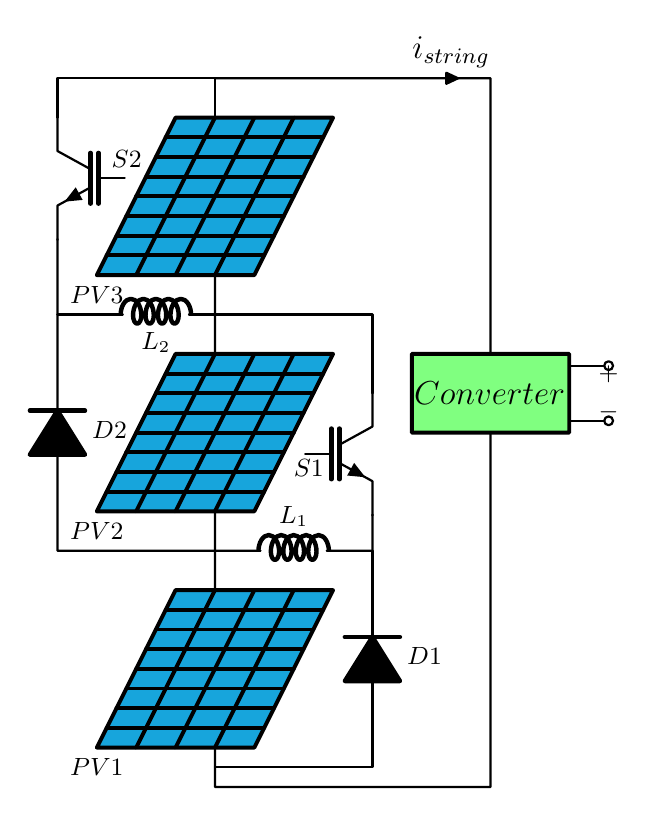
\begin{tikzpicture}
%Panel
	%Frame
	\draw (0,0) coordinate (P11);
	\draw (P11)++(2,0) coordinate(P12);
	\draw (P11)++(-1,-2) coordinate (P13);
	\draw (P13)++(2,0) coordinate(P14);
	\draw [line width=.5mm, fill=cyan!90!black] (P11)--(P12)--(P14)--(P13)--cycle;
	%-Horizontal Lines
	\draw [line width=.5mm] (P11)++ (-.125,-0.25)--++(2,0) ;
	\draw [line width=.5mm] (P11)++ (-.25,-0.5)--++(2,0);
	\draw [line width=.5mm] (P11)++ (-.375,-0.75)--++(2,0) ;
	\draw [line width=.5mm] (P11)++ (-.5,-1)--++(2,0) ;
	\draw [line width=.5mm] (P11)++  (-.625,-1.25)--++(2,0) ;
	\draw [line width=.5mm] (P11)++ (-.75,-1.5)--++(2,0)  ;
	\draw [line width=.5mm] (P11)++  (-.875,-1.75)--++(2,0) coordinate (P134) ;
	%Vertical Line
	\draw [line width=.5mm](P11)++(.5,0)--++(-1,-2);
	\draw [line width=.5mm] (P11)++(1,0)--++(-1,-2);
	\draw [line width=.5mm] (P11)++ (1.5,0)--++(-1,-2);
	\draw (P13)++(0,-0.25) coordinate (Pname1);
	\node (PVname1) at (Pname1) {$PV3$};

%Panel2
	%Frame
	\draw (0,-3) coordinate (P21);
	\draw (P21)++(2,0) coordinate(P22);
	\draw (P21)++(-1,-2) coordinate (P23);
	\draw (P23)++(2,0) coordinate(P24);
	\draw [line width=.5mm, fill=cyan!90!black] (P21)--(P22)--(P24)--(P23)--cycle;
	%Vertical Lines
	\draw [line width=.5mm] (P21)++ (-.125,-0.25)--++(2,0) ;
	\draw [line width=.5mm] (P21)++ (-.25,-0.5)--++(2,0) ;
	\draw [line width=.5mm] (P21)++ (-.375,-0.75)--++(2,0) ;
	\draw [line width=.5mm] (P21)++ (-.5,-1)--++(2,0) ;
	\draw [line width=.5mm] (P21)++  (-.625,-1.25)--++(2,0) ;
	\draw [line width=.5mm] (P21)++ (-.75,-1.5)--++(2,0)  ;
	\draw [line width=.5mm] (P21)++  (-.875,-1.75)--++(2,0) coordinate (P234) ;
	%Horizontal Line
	\draw [line width=.5mm] (P21)++(.5,0)--++(-1,-2);
	\draw [line width=.5mm] (P21)++(1,0)--++(-1,-2);
	\draw [line width=.5mm] (P21)++ (1.5,0)--++(-1,-2);
	\draw (P23)++(0,-0.25) coordinate (Pname2);
	\node (PVname2) at (Pname2) {$PV2$};

%Panel3
	%Frame
	\draw (0,-6) coordinate (P31);
	\draw (P31)++(2,0) coordinate(P32);
	\draw (P31)++(-1,-2) coordinate (P33);
	\draw (P33)++(2,0) coordinate(P34);
	\draw [line width=.5mm, fill=cyan!90!black] (P31)--(P32)--(P34)--(P33)--cycle;
	%Vertical Lines
	\draw [line width=.5mm] (P31)++ (-.125,-0.25)--++(2,0) ;
	\draw [line width=.5mm] (P31)++ (-.25,-0.5)--++(2,0) ;
	\draw [line width=.5mm] (P31)++ (-.375,-0.75)--++(2,0) ;
	\draw [line width=.5mm] (P31)++ (-.5,-1)--++(2,0) ;
	\draw [line width=.5mm] (P31)++ (-.625,-1.25)--++(2,0) ;
	\draw [line width=.5mm] (P31)++ (-.75,-1.5)--++(2,0) ;
	\draw [line width=.5mm] (P31)++ (-.875,-1.75)--++(2,0) coordinate (P334) ;
	%Horizontal Line
	\draw [line width=.5mm] (P31)++(.5,0)--++(-1,-2);
	\draw [line width=.5mm] (P31)++(1,0)--++(-1,-2);
	\draw [line width=.5mm] (P31)++ (1.5,0)--++(-1,-2);
	\draw (P33)++(0,-0.25) coordinate (Pname3);
	\node (PVname3) at (Pname3) {$PV1$};
	%Connections
	\draw (P31)++(0.5,0) coordinate (P3u); %P3 up connection
	\draw (P34)++(-0.5,0) coordinate (P3b); %P3 bottom connection
	\draw (P24)++(-0.5,0) coordinate (P2b); %P2 bottom connection
	\draw (P21)++(0.5,0) coordinate (P2u);  %P2 up connection
	\draw (P11)++(0.5,0) coordinate (P1u); %P1 up connection
	\draw (P14)++(-0.5,0) coordinate (P1b); %P1 bottom connection
	\draw (P3u)--(P2b);
	\draw (P14)++(-0.5,0) coordinate (P1b);
	\draw (P2u)--(P1b);
%Diodes and Switches
	%S1
	\draw (P3u)++(0,0.5) coordinate (P32m);
	\draw (P2u)++(0,0.5) coordinate (P21m);
	\draw (P21m)--++(2,0)--++(0,-1) node [nigbt, anchor=C , label={[xshift=-23, yshift=-12] $S1$ }] (nigbt12){};
	%D3
	\draw (P3b)++(0,-0.25) coordinate (P31m);
	\draw (P31m) --++(2,0) to [D*,l_=$D1$]++(0,2.75) coordinate(D3u) ;
	\draw (P32m) to [L, l=$L_1$] (D3u);
	\draw (nigbt12.E) to [short](D3u);
	\draw (P32m) to [short]++(-2,0) to [D*, l_=$D2$]++(0,3) coordinate(D2u);
	\draw (D2u) --++(0.5,0) to [L, l_=$L_2$] (P21m);
	\draw (P1u)--++(0,.5) coordinate (P1uu)--++(-2,0)--++(0,-0.5) node [nigbt, xscale=-1,  anchor=C , label={[xshift=25, yshift=0] $S2$ }] (nigbt11){};
	\draw (nigbt11.E) to [short](D2u);
	%Converter
	\draw (P1uu) --++(2.5,0) to [short,i=\large$ i_{string}$]++(1,0)--++(0,-3.5) coordinate(CMu);
	\draw (CMu)++(-1,-.5) coordinate (CMl);
	\draw (CMl)++(1,-.5) coordinate (CMb);
	\draw (CMb)++(1,0.15) coordinate (CO2);
	\draw (CO2)++(0,0.7) coordinate (CO1);
	\draw [line width=.5mm, fill=green!50] (CMu)--++(-1,0)--(CMl)-- ++(0,-0.5)--(CMb)--++(1,0)--(CO2)--(CO1)--++(0,0.15)--cycle;
	\draw (P3b)--++(0,-0.5)--++(3.5,0)--(CMb);
	\draw (CMl)++(-.1,0) coordinate (CMl1);
	\node [right] (Conv) at (CMl1) {\large $Converter$};
	%
	\draw (CO1)--++(0.5,0) to [open,o-o,v=$ $]++(0,-0.7)--(CO2);
\end{tikzpicture}
\end{document} 
